%%%%%%%%%%%%%%%%%%%%%%%%%%%%%%%%%%%%%%%%%%%%%%%%%%%%%%%%
%%%%%%%%%%%%%%%%%%%%%%%%%%%%%%%%%%%%%%%%%%%%%%%%%%%%%%%%
\section{Survival Analysis}
\label{additional:Survival}

Survival analysis is a subfield of statistics which examines problems involving the timing of events
such as death, component failure, or exiting a line of therapy after an adverse effect, in a population of subjects under study.
Using the appropriate models, quantities such as the lifetime, or failure rate, of a subject
can be estimated, as well as their dependence on other independent variables.
A variety of common models are available,
each with their own assumptions, capabilities, and limitations,
which make them best suited for certain applications.

%%%%%%%%%%%%%%%%%%%%%%%%%%%%%%%%%%%%%%%%%%%%%%%%%%%%%%%%
\subsection{Nomenclature}
\label{additional:Survival:Nomenclature}

\begin{symbollist}
	\item[Event] The event of interest in a study, \eg death, component failure\ldots
	\item[$t$] Time from the start of observation to an event, the conclusion of the study, or the withdrawal of a subject.
	\item[$T$] Time that an event occurred.
	\item[$x$] Independent variable(s) under consideration.
	\item[Censoring] Right\footnote{Left censored subjects enter the study after the event of interest has already occurred at an unknown $t < 0$.} censored subjects have no events during the observation period, either due to early withdrawal or the conclusion of the study. The true lifetime of these subjects is unavailable for analysis, \ie they have been censored.
	\item[$S\left(t\right)$] The survival function $S\left(t\right)$ is the probability that a subject survives longer than $t$, \ie $S\left(t\right) = P\left(T > t\right)$.
	\item[$F\left(t\right)$] The lifetime distribution function $F\left(t\right)$ is the complement of the survival function, \ie $F\left(t\right) = 1 - S\left(t\right) = P\left(T \leq t\right)$.
	\item[$f\left(t\right)$] The event density function $f\left(t\right)$ is the time derivative of the lifetime distribution function $F\left(t\right)$, $f\left(t\right) = \frac{dF}{dt} = -\frac{dS}{dt}$, if it exists.
	\item[$\lambda\left(t\right)$] The hazard function $\lambda\left(t\right)$ is the event rate at $t$ conditional on survival to time $t$, \ie $T > t$, see \cref{eq:Survival:hazard_def}. Any $\lambda\left(t\right)$ can be a hazard function, provided it satisfies \cref{eq:Survival:hazard_cond}.
	\item[$\Lambda\left(t\right)$] The cumulative hazard function $\Lambda\left(t\right)$ is the integral of $\lambda\left(t\right)$ with respect to time \cref{eq:Survival:cum_hazard:def}. Also see the relations in \cref{eq:Survival:cum_hazard:to_lambda,eq:Survival:cum_hazard:to_S}.
	\item[HR] The hazard ratio (HR) compares the hazards of two subsets of subjects partitioned by $x$ at time $t$, $\text{HR} = \lambda\left(x = 1\right) / \lambda\left(x=0\right)$. % TODO different from relative risk, also talk about log hazard
\end{symbollist}

\begin{subequations}\label{eq:Survival:hazard_def}
\begin{align}
\lambda\left(t\right) dt &= P\left(T \leq t + dt \mid T > t\right),\,\text{as} \,\, dt \to 0 \label{eq:Survival:hazard_def:a} \\
\lambda\left(t\right) &= \lim_{dt \to 0} \frac{P\left(T \leq t + dt \cap T > t\right)}{P\left(T > t\right)\,dt} \label{eq:Survival:hazard_def:b} \\
&= \frac{1}{S\left(t\right)} \lim_{dt \to 0} \frac{P\left(t < T \leq t + dt\right)}{dt} \label{eq:Survival:hazard_def:c} \\
&= \frac{1}{S\left(t\right)} \lim_{dt \to 0} \frac{F\left(t + dt\right) - F\left(t\right)}{dt} \label{eq:Survival:hazard_def:d} \\
&= \frac{f\left(t\right)}{S\left(t\right)} = -\frac{1}{S} \frac{dS}{dt} \label{eq:Survival:hazard_def:e}
\end{align}
\end{subequations}

\begin{subequations}\label{eq:Survival:hazard_cond}
\begin{gather}
\forall t \geq 0, \, \lambda\left(t\right) \geq 0 \label{eq:Survival:hazard_cond:a} \\
\int_{0}^{\infty} \lambda\left(t\right) \, \dif t = \infty \label{eq:Survival:hazard_cond:b}
\end{gather}
\end{subequations}

\begin{subequations}\label{eq:Survival:cum_hazard}
\begin{gather}
\Lambda\left(t\right) = \int_{0}^{t} \lambda\left(u\right) \, \dif u = - \ln\left(S\left(t\right)\right) \label{eq:Survival:cum_hazard:def} \\
\lambda\left(t\right) = \frac{d\Lambda}{dt} = -\frac{1}{S} \frac{dS}{dt} \label{eq:Survival:cum_hazard:to_lambda} \\
S\left(t\right) = \exp\left(-\Lambda\left(t\right)\right) \label{eq:Survival:cum_hazard:to_S}
\end{gather}
\end{subequations}

\subsubsection{Expected Future Lifetime}
\label{additional:Survival:Nomenclature:efl}
The expected future lifetime $\expval{T-t_{0}}$ is the
expected additional time of survival for a subject having already survived to $t_{0}$.
We can derive $\expval{T-t_{0}}$ \cref{eq:Survival:efl_der:efl}
from the probability of an event occurring between $t_{0}$ and $t_{0} + t$ \cref{eq:Survival:efl_der:P}
using the prior work of \cref{eq:Survival:hazard_def} and integration by parts:

\begin{subequations}\label{eq:Survival:efl_der}
\begin{gather}
P\left(T \leq t_{0} + t \mid T > t_{0}\right)
= \frac{F\left(t_{0} + t\right) - F\left(t_{0}\right)}{S\left(t_{0}\right)} \label{eq:Survival:efl_der:P} \\
\text{PDF}
= \frac{d}{dt} P\left(T \leq t_{0} + t \mid T > t_{0}\right)
= \frac{f\left(t_{0} + t\right)}{S\left(t_{0}\right)} \label{eq:Survival:efl_der:pdf} \\
\expval{T-t_{0}}
= \int_{0}^{\infty} t \, \text{PDF} \, \dif t
= \frac{1}{S\left(t_{0}\right)} \int_{0}^{\infty} S\left(t\right) \, \dif t \label{eq:Survival:efl_der:efl}
\end{gather}
\end{subequations}

%%%%%%%%%%%%%%%%%%%%%%%%%%%%%%%%%%%%%%%%%%%%%%%%%%%%%%%%
\subsection{Kaplan-Meier Model}
\label{additional:Survival:KM}

The Kaplan-Meier model $\hat{S}_{\text{KM}}\left(t\right)$ is a non-parametric estimate of $S\left(t\right)$ computed from empirical data.

\begin{equation}\label{eq:Survival:KM}
\hat{S}_{\text{KM}}\left(t\right) = \prod_{i:\,t_{i} < t} \left(1 - \frac{d_{i}}{n_{i}}\right)
\end{equation}

\noindent Here the product is over all times $t_{i}$ at which $d_{i}$ events occurred,
and $n_{i}$ is the number of subjects still under study at $t_{i}$,
\ie subjects who have not had an event or been censured.
Due to its construction, $\hat{S}_{\text{KM}}\left(t\right)$ remains steady
between $t_{i}$ but drops vertically at each data point.
Therefore the derivative does not exist and we can not estimate $f\left(t\right)$ or $\lambda\left(t\right)$.


We can apply the Kaplan-Meier estimator to different subsets of subjects partitioned by a categorical variable $x$
in order to understand the dependence of $S\left(t\right)$ on $x$.
Note that $x$ can not be a continuous variable, and must be binned to integer classes if that is the case.

A simple example in \R utilizing the built in Acute myeloid leukemia (aml) dataset is provided below.
The status variable represents the event, recurrence of leukemia, as $\text{status}=1$, and the censoring of a patient as $\text{status}=0$.
Two different treatment paths are present in the data, $x=$ Maintained and Nonmaintained.

\begin{figure}[H]
\centering
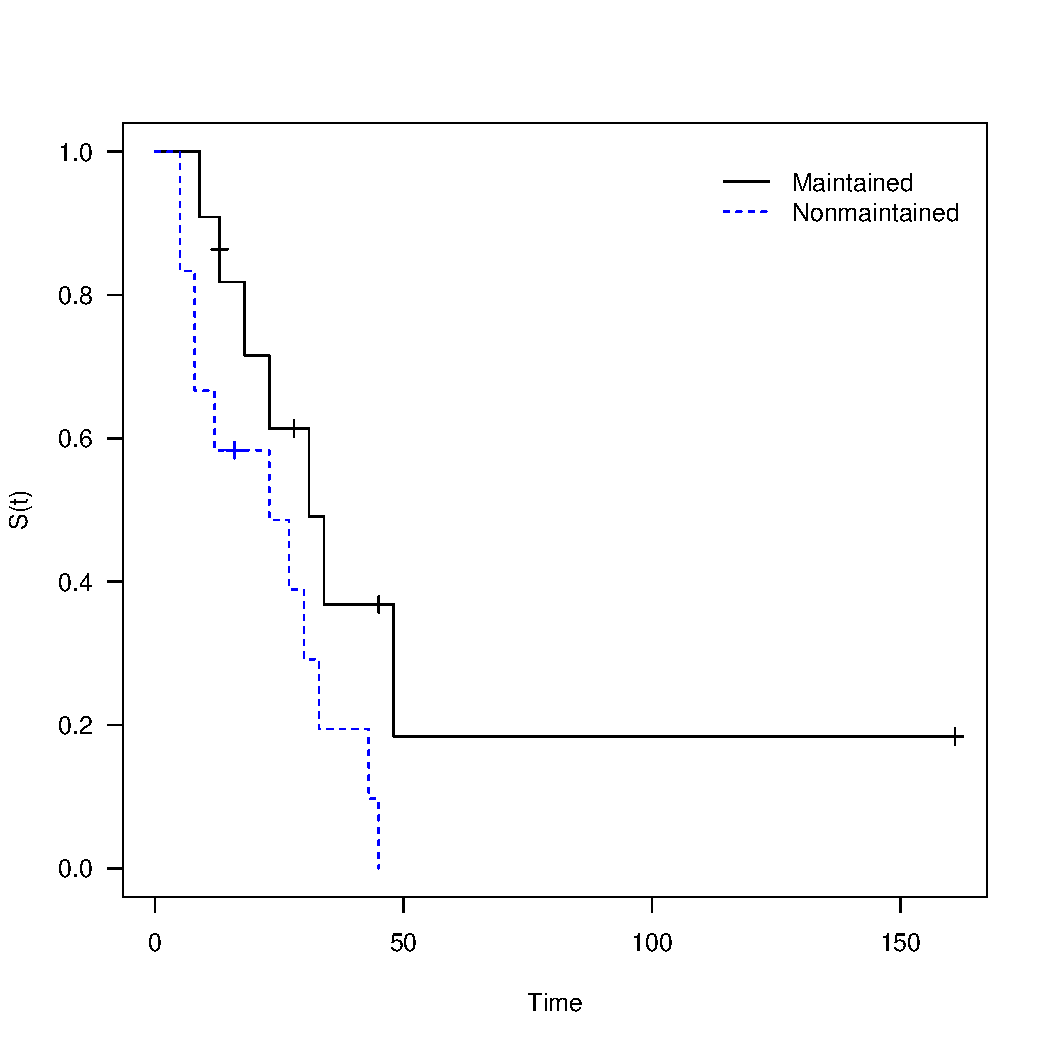
\includegraphics[width=0.7\textwidth]{figures/survival/aml_km.pdf}
\vspace{0.2cm}
\caption{
Kaplan-Meier plot of the aml dataset. Censoring events are displayed with tick marks.
}
\label{fig:aml_km}
\end{figure}

% TODO move R into own section, add other model examples to code and plot
\begin{lstlisting}[language=R]
> library(survival)
> aml[with(aml, order(time)), ]
   time status             x
12    5      1 Nonmaintained
13    5      1 Nonmaintained
14    8      1 Nonmaintained
15    8      1 Nonmaintained
1     9      1    Maintained
16   12      1 Nonmaintained
2    13      1    Maintained
3    13      0    Maintained
17   16      0 Nonmaintained
4    18      1    Maintained
5    23      1    Maintained
18   23      1 Nonmaintained
19   27      1 Nonmaintained
6    28      0    Maintained
20   30      1 Nonmaintained
7    31      1    Maintained
21   33      1 Nonmaintained
8    34      1    Maintained
22   43      1 Nonmaintained
9    45      0    Maintained
23   45      1 Nonmaintained
10   48      1    Maintained
11  161      0    Maintained
> km.model <- survfit(Surv(time, status) ~ x, data=aml, type="kaplan-meier")
> summary(km.model)
Call: survfit(formula = Surv(time, status) ~ x, data = aml, type = "kaplan-meier")

                x=Maintained
 time n.risk n.event survival std.err lower 95% CI upper 95% CI
    9     11       1    0.909  0.0867       0.7541        1.000
   13     10       1    0.818  0.1163       0.6192        1.000
   18      8       1    0.716  0.1397       0.4884        1.000
   23      7       1    0.614  0.1526       0.3769        0.999
   31      5       1    0.491  0.1642       0.2549        0.946
   34      4       1    0.368  0.1627       0.1549        0.875
   48      2       1    0.184  0.1535       0.0359        0.944

                x=Nonmaintained
 time n.risk n.event survival std.err lower 95% CI upper 95% CI
    5     12       2   0.8333  0.1076       0.6470        1.000
    8     10       2   0.6667  0.1361       0.4468        0.995
   12      8       1   0.5833  0.1423       0.3616        0.941
   23      6       1   0.4861  0.1481       0.2675        0.883
   27      5       1   0.3889  0.1470       0.1854        0.816
   30      4       1   0.2917  0.1387       0.1148        0.741
   33      3       1   0.1944  0.1219       0.0569        0.664
   43      2       1   0.0972  0.0919       0.0153        0.620
   45      1       1   0.0000     NaN           NA           NA

> pdf('~/aml_km.pdf')
> plot(km.model, conf.int=F, xlab='Time', ylab='S(t)', col=c('black', 'blue'), las=1, mark.time=T, lty=1:2, las=1)
> legend(110, 1, c('Maintained', 'Nonmaintained'), col=c('black', 'blue'), lty=1:2, bty='n')
> dev.off()
\end{lstlisting}

%%%%%%%%%%%%%%%%%%%%%%%%%%%%%%%%%%%%%%%%%%%%%%%%%%%%%%%%
\subsection{Exponential Model}
\label{additional:Survival:exp}
The exponential model is a parametric estimate of $S\left(t\right)$
valid when the hazard is expected to be constant with respect to $t$.
In nuclear physics\footnote{$\frac{dN}{dt} = -\lambda N$, $N\left(t\right) = N_{0} e^{-\lambda t}$, half-life $t_{1/2} = \ln\left(2\right) / \lambda = \tau \ln\left(2\right)$, where $\tau$ is the time constant.} $\lambda\left(t\right) = \lambda$
decays per unit time really is a constant.
However, in most situations $\lambda = c$ is unrealistic over longer time scales.
The exponential model can accommodate both categorical and continuous $x$ independent variables.

The survival function for the exponential model is simply

\begin{equation}\label{eq:Survival:exp}
\hat{S}_{\text{Exp}}\left(t\right) = e^{-\lambda t}
\end{equation}

\noindent where the hazard can be expanded in terms of $\mathbf{x}$, $\bm{\beta}$ as in a regression analysis:

\begin{equation}\label{eq:Survival:exp_lambda}
\begin{aligned}
\lambda\left(x\right) &= \exp\left(\beta_{0} + \sum_{j=1}^{n}\, \beta_{j} x_{j}\right) \\
\log\left(\lambda\right) &= \mathbf{x} \bm{\beta}
\end{aligned}
\end{equation}

\noindent Here we are making the {\em proportional hazards assumption},
\ie the differences in $\lambda$ between subgroups in $x_{j}$
are proportional\footnote{Really $\log\left(\lambda\right) \propto \beta$.} to $\beta_{j}$
and constant over $t$.

The hazard ratio for $x_{j}$ is then:

\begin{equation}\label{eq:Survival:exp_HR}
\begin{aligned}
\text{HR}_{\text{Exp}} &= e^{\ldots+\beta_{j} 1+\ldots} / e^{\ldots+\beta_{j} 0+\ldots} \\
&= e^{\beta_{j}}
\end{aligned}
\end{equation}

\subsubsection{Weibull Model}
\label{additional:Survival:weibull}
The Weibull model expands on the standard exponential model
by introducing a shape parameter $k$ to adjust the time dependence of the hazard:

\begin{equation}\label{eq:Survival:weibull}
\begin{aligned}
\hat{S}_{\text{Weibull}}\left(t\right) &= e^{-\lambda_{\text{Weibull}} t} \\
\lambda_{\text{Weibull}} &= \exp\left(\beta_{0} t^{k} + \sum_{j=1}^{n}\, \beta_{j} x_{j}\right) \\
\text{HR}_{\text{Weibull}} &= e^{\beta_{j}}
\end{aligned}
\end{equation}

\noindent Here $\beta_{0}$ is the scale parameter of the hazard with respect to $t$,
while the other $\beta_{j}$ are scale parameters for the independent $x_{j}$.
For $k<0$ ($k>0$) the hazard monotonically decreases (increases) over time,
while $k=0$ returns the exponential model.
This allows phenomena such as burn in and compounding component failures to be modeled.
Numerous parameterizations and expansions of the Weibull model are available,
however they all share the property that
$\lambda = \exp\left(\beta_{0} f\left(t\right) + \sum_{j=1}^{n}\, \beta_{j} x_{j}\right)$
where $f\left(t\right)$ is a {\em known}, almost always monotonic, function of $t$.

%%%%%%%%%%%%%%%%%%%%%%%%%%%%%%%%%%%%%%%%%%%%%%%%%%%%%%%%
\subsection{Cox Proportional-Hazards Model}
\label{additional:Survival:cox}
The Cox proportional-hazards model is a
semiparametric\footnote{Semiparametric as $\lambda_{0}\left(t\right)$ is unknown, but $\bm{\beta}$ are still parameters of $\lambda$.} model
which further expands on the Weibull model by allowing
the time dependence of $\lambda$ to be an unknown function.
As the name suggests, the proportional hazards assumption is retained
allowing us to compute useful HR values
without even knowing $\lambda\left(t\right)$ or $S\left(t\right)$.

In the Cox model we assume the hazard has the form of

\begin{equation}\label{eq:Survival:cox_lambda}
\lambda_{\text{Cox}} = \lambda_{0}\left(t\right) \exp\left(\sum_{j=1}^{n}\, \beta_{j} x_{j}\right)
\end{equation}

\noindent where $\lambda_{0}\left(t\right)$ is an unknown function of $t$.
When computing hazard ratios $\lambda_{0}\left(t\right)$ then drops out:

\begin{equation}\label{eq:Survival:cox_HR}
\text{HR}_{\text{Exp}} = e^{\beta_{j}}
\end{equation}

% TODO

\subsubsection{Assumptions}
\label{additional:Survival:cox:assumptions}
% TODO

%%%%%%%%%%%%%%%%%%%%%%%%%%%%%%%%%%%%%%%%%%%%%%%%%%%%%%%%
\subsection{Method Comparison}
\label{additional:Survival:comp}
% TODO

\begin{table}[H]
\centering
\begin{tabular}{l|l|l}
\multicolumn{1}{c|}{Kaplan-Meier} & \multicolumn{1}{c|}{Exponential / Weibull} & \multicolumn{1}{c}{Cox} \\
\cline{1-3}
\begin{tabular}[c]{p{0.3\textwidth}}
Pro
\begin{itemize}
	\item Simple to compute and understand
	\item Can estimate $S$
\end{itemize}
\\
Con
\begin{itemize}
	\item No functional form
	\item Can \textbf{not} estimate HR
	\item Only can handle a few categorical $x$
\end{itemize}
\end{tabular}

&

\begin{tabular}[c]{p{0.3\textwidth}}
Pro
\begin{itemize}
	\item Can estimate $S$ and HR
\end{itemize}
\\
Con
\begin{itemize}
	\item $\lambda\left(t\right) = c$ can be unrealistic
	\item Weibull: $\lambda = f\left(t\right)$ of a known form
\end{itemize}
\end{tabular}

&

\begin{tabular}[c]{p{0.3\textwidth}}
Pro
\begin{itemize}
	\item $\lambda$ can be an unknown function of $t$
	\item Can estimate HR
\end{itemize}
\\
Con
\begin{itemize}
	\item Can \textbf{not} estimate $S$
\end{itemize}
\end{tabular}

\\
\end{tabular}
\end{table}

%%%%%%%%%%%%%%%%%%%%%%%%%%%%%%%%%%%%%%%%%%%%%%%%%%%%%%%%
\subsection{}
\label{additional:Survival:}
% TODO

% TODO survdiff(Surv(time, status) ~ x, data=aml)
% TODO common assumptions, censuring is non-informative, \ie uncorrelated with event outcome
